\usepackage{physics}
\usepackage{amsmath}
\usepackage{tikz}
\usepackage{mathdots}
\usepackage{yhmath}
\usepackage{cancel}
\usepackage{color}
\usepackage{siunitx}
\usepackage{array}
\usepackage{multirow}
\usepackage{amssymb}
\usepackage{gensymb}
\usepackage{tabularx}
\usepackage{extarrows}
\usepackage{booktabs}
\usetikzlibrary{fadings}
\usetikzlibrary{patterns}
\usetikzlibrary{shadows.blur}
\usetikzlibrary{shapes}




\tikzset{every picture/.style={line width=0.75pt}} %set default line width to 0.75pt        

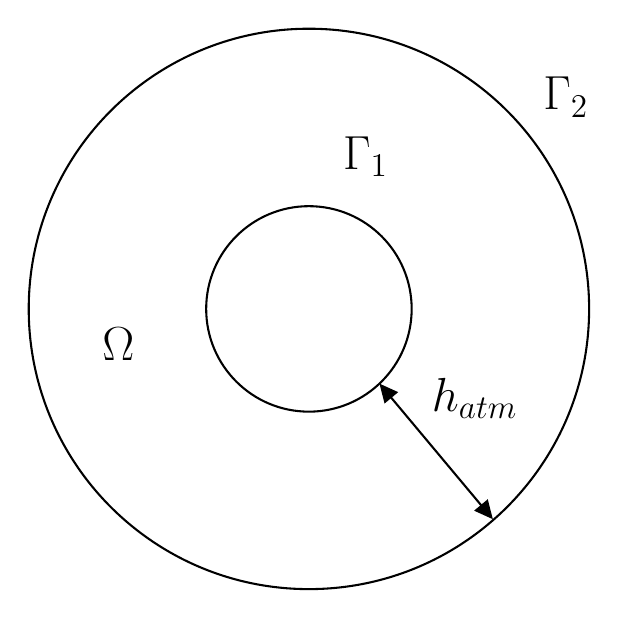
\begin{tikzpicture}[x=0.75pt,y=0.75pt,yscale=-1,xscale=1]
%uncomment if require: \path (0,300); %set diagram left start at 0, and has height of 300

%Shape: Circle [id:dp19457056715612908] 
\draw   (225,152) .. controls (225,77.44) and (285.44,17) .. (360,17) .. controls (434.56,17) and (495,77.44) .. (495,152) .. controls (495,226.56) and (434.56,287) .. (360,287) .. controls (285.44,287) and (225,226.56) .. (225,152) -- cycle ;
%Shape: Circle [id:dp44598804607922415] 
\draw   (310.5,152) .. controls (310.5,124.66) and (332.66,102.5) .. (360,102.5) .. controls (387.34,102.5) and (409.5,124.66) .. (409.5,152) .. controls (409.5,179.34) and (387.34,201.5) .. (360,201.5) .. controls (332.66,201.5) and (310.5,179.34) .. (310.5,152) -- cycle ;
%Straight Lines [id:da4358574767339618] 
\draw    (395.92,190.3) -- (446.68,251) ;
\draw [shift={(448.6,253.3)}, rotate = 230.1] [fill={rgb, 255:red, 0; green, 0; blue, 0 }  ][line width=0.08]  [draw opacity=0] (8.93,-4.29) -- (0,0) -- (8.93,4.29) -- cycle    ;
\draw [shift={(394,188)}, rotate = 50.1] [fill={rgb, 255:red, 0; green, 0; blue, 0 }  ][line width=0.08]  [draw opacity=0] (8.93,-4.29) -- (0,0) -- (8.93,4.29) -- cycle    ;

% Text Node
\draw (375,67.4) node [anchor=north west][inner sep=0.75pt]  [font=\LARGE]  {$\Gamma _{1}$};
% Text Node
\draw (471.5,38.9) node [anchor=north west][inner sep=0.75pt]  [font=\LARGE]  {$\Gamma _{2}$};
% Text Node
\draw (259,159.4) node [anchor=north west][inner sep=0.75pt]  [font=\LARGE]  {$\Omega $};
% Text Node
\draw (417.8,184) node [anchor=north west][inner sep=0.75pt]  [font=\LARGE]  {$h_{atm}$};


\end{tikzpicture}
